\documentclass[10pt]{beamer}

\usepackage[T2A]{fontenc}
\usepackage[utf8]{inputenc}
\usepackage[russian,english]{babel}

\usefonttheme[onlymath]{serif}

\usetheme[progressbar=frametitle]{metropolis}
\usepackage{appendixnumberbeamer}

\usepackage{booktabs}
\usepackage[scale=2]{ccicons}

\usepackage{pgfplots}
\usepgfplotslibrary{dateplot}

\usepackage{xspace}
\newcommand{\themename}{\textbf{\textsc{metropolis}}\xspace}
\newcommand{\TODO}[1]{\textbf{\textcolor{red}{TODO: #1}}}

\date{}
\author{Екатерина Тузова}


\title{Лекция 4}
\subtitle{Деревья принятия решений}

\begin{document}

\maketitle

\section{Разбор летучки}

\section{Мотивирующий пример}
{\foot{\href{https://www.kaggle.com/alopez247/pokemon}{Pokémon for Data Mining and Machine Learning (https://www.kaggle.com/alopez247/pokemon)}}
\begin{frame}{Мотивирующий пример}
	\begin{figure}
	    \centering
	    \subfloat{{
\includegraphics[width=2cm]{../lecture2/images/Bulbasaur} }}
	    \qquad
	    \subfloat{{
\includegraphics[width=2cm]{../lecture2/images/Mewtwo} }}
    	    \qquad
    	    \subfloat{{
\includegraphics[width=2cm]{../lecture2/images/Volcanion} }}
    	    \qquad
    	    \subfloat{{
\includegraphics[width=2cm]{../lecture2/images/Ekans} }}
    	    \qquad
    	    \subfloat{{
\includegraphics[width=2cm]{../lecture2/images/Nidorina} }}
	    \qquad 
    	    \subfloat{{
\includegraphics[width=2cm]{../lecture2/images/Rattata} }}
	    \qquad
    	    \subfloat{{
\includegraphics[width=2cm]{../lecture2/images/Sandshrew} }}
	    \qquad
    	    \subfloat{{
\includegraphics[width=2cm]{../lecture2/images/Articuno} }}    	        	    
	\end{figure}
\end{frame}
}

\begin{frame}{Датасет}
    \centering
	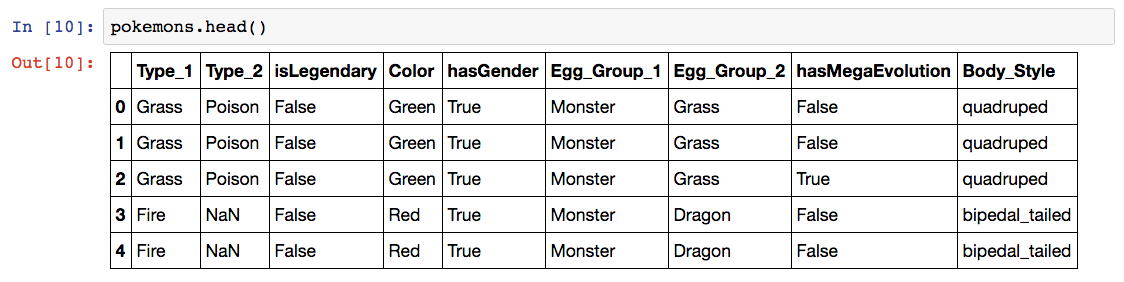
\includegraphics[width=\textwidth]{images/pokemons}
\end{frame}

\begin{frame}{Мотивация}
    \centering
	
\includegraphics[width=\textwidth, height=0.8 \textheight, keepaspectratio]{images/distance}
\end{frame}

\begin{frame}{Логические закономерности}
	${X^l = \left( x_i, y_i \right)_{i=1}^l}$ - обучающая выборка.\\
	\bigbreak
	\alert{Логическая закономерность} -- предикат ${\beta: X \rightarrow \left\{ 0, 1 \right\} }$, который удовлетворяет двум требованиям:\\
	\pause
	\begin{enumerate} 
		\item Интерпретируемость
		\pause
		\item Информативность относительно одного из классов ${c \in Y}$
	\end{enumerate}
\end{frame}

\begin{frame}{Логические закономерности}
	${X^l = \left( x_i, y_i \right)_{i=1}^l}$ - обучающая выборка.\\
	\bigbreak
  Предикат ${\beta: X \rightarrow \left\{ 0, 1 \right\} }$\\
	\bigbreak
	\alert{Алгоритм}: $a(X, \beta) \rightarrow y$
\end{frame}

\begin{frame}{Интерпретируемость}
	\begin{enumerate}
		\item Записывается на естественном языке
		\item Зависит от небольшого числа признаков
	\end{enumerate}
\end{frame}

\begin{frame}{Примеры}
	Медицинская диагностика:	
		\begin{enumerate} [-]
			\item Температура выше $n^\circ$
			\item Есть ли кашель
		\end{enumerate}
	\bigbreak
	Кредитный скоринг:	
		\begin{enumerate} [-]
			\item Заработная плата выше, чем $n$ руб.
			\item Кредит не больше, чем $m$ руб.
		\end{enumerate}
\end{frame}

\begin{frame}{Интерпретируемость}
    \centering
	
\includegraphics[width=\textwidth, height=0.8 \textheight, keepaspectratio]{images/decisiontree}
\end{frame}


\begin{frame}{Информативность}
  \alert{Идея}: Максимизировать количество правильно распознанных объектов класса $c$ и при этом минимизировать количество объектов, ошибочно классифицированных как класс $c$
  \pause
	\bigbreak
	$${ tp(\beta) = \# \left\{ x_i: \beta(x_i) = 1 , y_i = c \right\} \rightarrow \max }$$\\
	\pause
  \bigbreak
	$${ fp(\beta) = \# \left\{ x_i: \beta(x_i) = 1 , y_i \neq c \right\} \rightarrow \min }$$\\		
\end{frame}

\begin{frame}{Поиск закономерности}
	\begin{figure}[htbp]
	  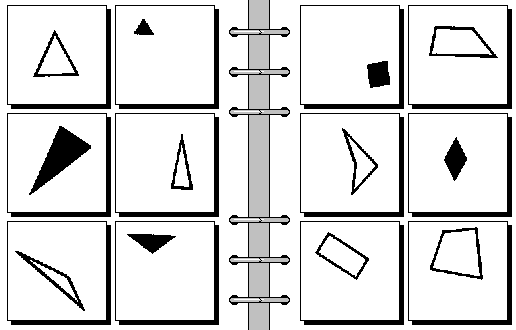
\includegraphics[height=150pt, keepaspectratio = true]{images/bongard6}   
	\end{figure}
\end{frame}

\begin{frame}{Поиск закономерности}
	\begin{figure}[htbp]
	  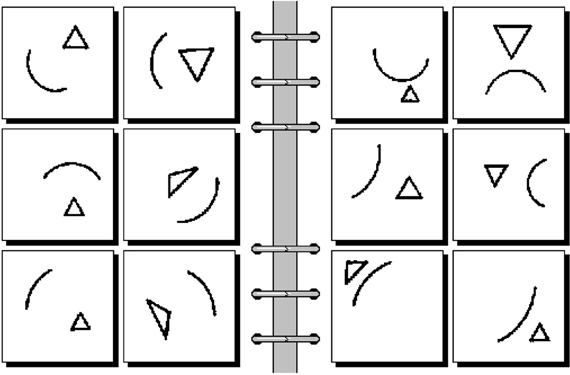
\includegraphics[height=150pt, keepaspectratio = true]{images/bongard40}   
	\end{figure}
\end{frame}

\begin{frame}{Поиск закономерности}
	\begin{figure}[htbp]
	  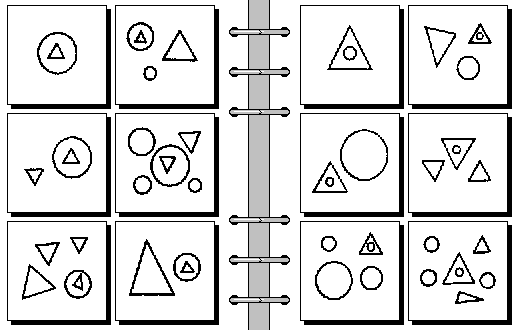
\includegraphics[height=150pt, keepaspectratio = true]{images/bongard47}   
	\end{figure}
\end{frame}

\begin{frame}{Поиск закономерности}
	\begin{figure}[htbp]
	  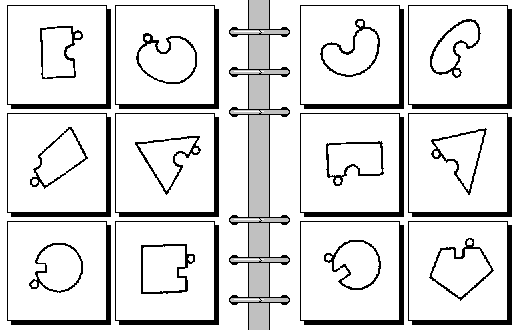
\includegraphics[height=150pt, keepaspectratio = true]{images/bongard55}   
	\end{figure}
\end{frame}

\begin{frame}{Основные вопросы}
	\begin{enumerate}
		\item Как изобретать признаки? 
		\item Какого вида закономерности $\beta(x)$ нужны?
		\item Как определять информативность? 
		\item Как выбирать закономерности?
		\item Как объединять закономерности в алгоритм?
	\end{enumerate}
\end{frame}

\section{Виды правил}

\begin{frame}{Виды правил}
	\begin{itemize} [<+->]
	\item[--] Пороговое условие\\
	$\beta(x) = \left[f_j(x) \leq a_j \right]$ или  $\left[a_j \leq f_j(x) \leq b_j \right]$
	\item[--] Конъюнкция из $J$ пороговых условий \\
	$\beta(x) = \bigwedge\limits_{j \in J} \left[a_j \leq f_j(x) \leq b_j \right]$
	\item[--] Синдром -- выполнение не менее $d$ условий из $J$
	$\beta(x) = \left[\sum\limits_{j \in J} \left[a_j \leq f_j(x) \leq b_j \right] \geq d \right]$
	\end{itemize}
\end{frame}

\begin{frame}{Оценивание информативности}
	\alert{Идея}: Хотим получить один критерий из двух:\\
	\bigbreak
	${ tp(\beta) = \# \left\{ x_i: \beta(x_i) = 1 , y_i = c \right\} \rightarrow \max  }$ 
	${ fp(\beta) = \# \left\{ x_i: \beta(x_i) = 1 , y_i \neq c \right\} \rightarrow \min}$ \\
	\bigbreak
	\pause
	Очевидные свертки:\\
	\begin{enumerate}
		\item $I(tp, fp) = \frac{tp}{tp+fp} \rightarrow \max$
		\item $I(tp, fp) = tp-fp \rightarrow \max$
		\item $I(tp, fp) = tp-Cfp \rightarrow \max$			
	\end{enumerate}
\end{frame}

\begin{frame}{Пример свертки двух критериев}
	Пусть число примеров искомого класса 200 и число остальных объектов 100\\
	\bigbreak
	\begin{tabular}{|r l|l|l|l|}
	  \hline 
	  $tp$ & $fp$ & $tp-fp$ & $tp-5fp$ & $\frac{tp}{tp+fp}$\\ 
	  \hline \hline
	  50 & 0 & \textcolor{red}{50} & 50 & 1\\
	  \hline
	  100 & 50 & \textcolor{red}{50} & -150 & 0.6\\
	  \hline \hline
	  50 & 9 & 41 & \textcolor{red}{5} & \textcolor{red}{0.84}\\
	  \hline  
	  5 & 0 & 5 & \textcolor{red}{5} & \textcolor{red}{1}\\  
	  \hline 
	\end{tabular}
\end{frame}

\section{Критерии информативности}

\begin{frame}{Энтропийный информационный критерий}
  \begin{align*} 
		IGain(tp,fp) &= h(\frac{P}{l}) - \frac{tp+tp}{l}h(\frac{tp}{tp+fp}) - \\
		&- \frac{l-tp-fp}{l}h(\frac{P-tp}{l-tp-fp}) \rightarrow \max \\
	\end{align*} 
	$h(q) = -q\log_2q - (1-q)\log_2(1-q)$
	\bigbreak	
	$P$ - общее количество объектов искомого класса\\
	$N$ -- количество остальных объектов
\end{frame}

\begin{frame}{Критерий Джини}
	$$IGini(tp,fp)=IGain(tp,fp) $$\\
	\bigbreak
	$h(q)=4q(1-q)$
	\bigbreak
	$P$ - общее количество объектов искомого класса\\
	$N$ -- количество остальных объектов
\end{frame}

{\foot{Fisher’s Exact Test}
\begin{frame}{Точный тест Фишера}
	$$IStat(tp,fp) = -\frac{1}{l}\log_2\frac{C_P^{tp}C_N^{fp}}{C_{P+N}^{tp+fp}} \rightarrow \max$$\\
	\bigbreak
	$P$ - общее количество объектов искомого класса\\
	$N$ -- количество остальных объектов
\end{frame}
}

\begin{frame}{Поиск информативных закономерностей}
  \begin{algorithmic}[1]
    \Function{find\_regularity}{$X^l$}
    \State Выбрать начальное множество $\mathcal{B}$
    \MRepeat [пока правила улучшаются] 
      \State $\mathcal{B}'=$ множество модификаций правил $\beta \in \mathcal{B}$
      \State Удалить слишком похожие правила из $\mathcal{B} \cup \mathcal{B}'$
      \State Оценить инфомативность правил $\beta \in \mathcal{B}'$
      \State $\mathcal{B}=$ наиболее информативные правила из $\mathcal{B} \cup \mathcal{B}'$
    \EndRepeat
  \EndFunction
  \end{algorithmic}    
\end{frame}

\begin{frame}
	\begin{enumerate}[--]
		\item Генетические алгоритмы
		\item Метод ветвей и границ	
		\item Стохастический локальный поиск	
	\end{enumerate}
\end{frame}

\begin{frame}{Критерий Парето}
  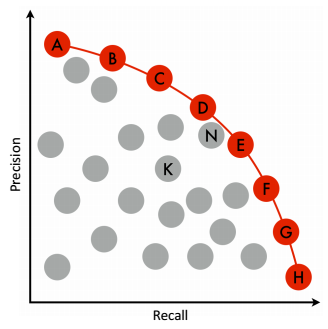
\includegraphics[height=150pt, keepaspectratio = true]{images/pareto}   \\
  Парето-фронт -- множество недоминируемых закономерностей
\end{frame}

\section{Как собрать классификатор из закономерностей?}

\begin{frame}{Решающий список}
	\alert{Идея}:\\
	Возьмем $\beta_1(x), \beta_2(x), \dots, \beta_T(x)$ закономерностей и будем по порядку применять на объекте. 
	Как только предикат $\beta_i$ сработал -- вернем соответствующий класс $c_i$.\\
	\bigbreak
	\pause
	$E(\beta_i, X^l) = \frac{fp(\beta_i)}{fp(\beta_i)+tp(\beta_i)} \rightarrow \min$ -- доля ошибок $\beta_i$ на $X^l$\\
	\bigbreak
	Т.к. каждое правило принимает окончательное решение $\Rightarrow$ ошибка правила равна ошибке всего алгоритма
\end{frame}

\begin{frame}{Жадный алгоритм для решающего списка}
  \begin{algorithmic}[1]
    \Function{decision\_list}{$X^l$, $\mathcal{B}$, $T_{max}$, $I_{min}$, $E_{max}$, $l_0$}
      \State $U \gets X^l$
	    \For {\textbf{each} $i = 1,2,\dots,T_{max}$}
	      \State Выбрать класс $c_i$
	      \State $\beta_i = \max\limits_{E(\beta, U) \leq E_{max}} I(\beta, U)$
	      \If {$I(\beta_i, U) < I_{min}$}
	        \State \textbf{continue}
	      \EndIf
	      \State $U = \left\{ x \in U: \beta_i(x) = 0 \right\}$
	      \If {$\vert U \vert \leq l_0$}
	        \Return
	      \EndIf
      \EndFor
    \EndFunction
  \end{algorithmic}    
\end{frame}

\begin{frame}{Наблюдения}
	\begin{enumerate}[--]
	\item Низкое качество классификации
	\item Разные стратегии выбора класса $c_i$
	\item Подбор параметров
	\end{enumerate}
	\bigbreak
	\pause
	Параметр $E_{max}$ влияет на сложность списка:\\
	$E_{max} \downarrow$ $\Rightarrow$ $tp(\beta_i) \downarrow$, $T \uparrow$\\
	$E_{max} \uparrow$ $\Rightarrow$ underfitting
\end{frame}


\begin{frame}{Бинарное решающее дерево}
	Бинарное решающее дерево -- алгоритм классификации $a(x, \beta)$, задающийся бинарным деревом:\\
	\begin{enumerate}[--]
	\item $\forall v \in V_{inner} \rightarrow \beta_v: X \rightarrow \left\{ 0,1\right\}$, $\beta \in \mathcal{B}$
	\item $\forall v \in V_{leaf} \rightarrow $ имя класса $c_v \in Y$\\
	
	\begin{figure}[htbp]
	  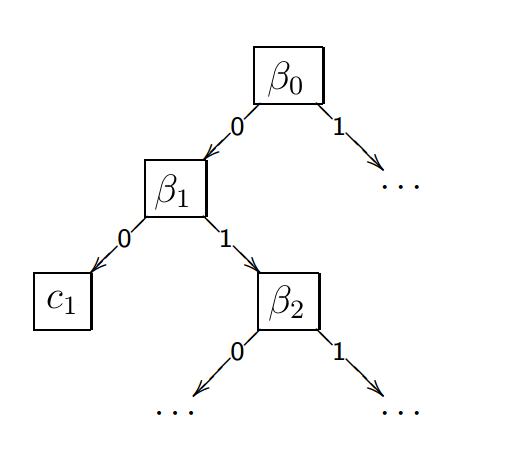
\includegraphics[height=150pt, keepaspectratio = true]{images/binary_tree}   
	\end{figure}
	\end{enumerate}
\end{frame}

\begin{frame}{Пример решающего дерева}
  \TODO{picture}
\end{frame}

{\foot{Iterative Dichotomizer 3}
\begin{frame}{Алгоритм построения ID3}
  \begin{algorithmic}[1]
    \Function{LearnID3}{$U$, $\mathcal{B}$}
       \If {все объекты из $U$ лежат в одном классе $c \in Y$}
         \State \Return {новый лист $v$, $c_v = c$}
       \EndIf
       \State $\beta^* = \max\limits_{\beta \in \mathcal{B}} I(\beta, U)$
       \State $U_0 = \left\{ x \in U : \beta^*(x) = 0\right\}$	
       \State $U_1 = \left\{ x \in U : \beta^*(x) = 1\right\}$	
       \If {$U_0 = \oslash$ или $U_1 = \oslash$}
         \State \Return {$v$, $c_v$ = Majority(U)}
       \EndIf
       \State Создать новую внутреннюю вершину $v$: $\beta_v = \beta^*$
       \State $L_v =$ LearnID3 ($U_0$, $\mathcal{B}$)
       \State $R_v =$ LearnID3 ($U_1$, $\mathcal{B}$)
       \State \Return $v$
    \EndFunction
  \end{algorithmic}    
\end{frame}
}

\section{Критерий информативности}

\begin{frame}{Критерий Джини}
  $$I(\beta,X^l)= \# \left\{ (x_i, x_j): \beta(x_i) = \beta(x_j), y_i = y_j \right\}$$
\end{frame}

\begin{frame}{Критерий Донского}
  $$I(\beta,X^l)= \# \left\{ (x_i, x_j): \beta(x_i) \neq \beta(x_j), y_i \neq y_j \right\}$$
\end{frame}

\begin{frame}{Плюсы}
	\begin{enumerate}[<+- |alert@+>] 
	\item[+] Интерпретируемость и простота классификации
	\item[+] Допустимы разнотипные данные и данные с пропусками
	\item[+] Не бывает отказов от классификации
	\item[+] Трудоёмкость линейна по длине выборки
	\item[+] Можно варьировать множество $\mathcal{B}$
	\end{enumerate}
\end{frame}

\begin{frame}{Минусы}
	\begin{enumerate} [<+- |alert@+>] 
	\item[--] Жадный ID3 сильно переобучается
	\item[--] Высокая чувствительность к шуму, к составу выборки, к критерию информативности
	\item[--] Чем дальше $v$ от корня, тем меньше надёжность выбора $\beta_v$ , $c_v$
	\end{enumerate}
\end{frame}

\begin{frame}{Переобучение}
\TODO{picture}
\end{frame}

\begin{frame}{Подрезание дерева C4.5}
  $X^k$ -- независимая контрольная выборка, $k \approx 0.5l$\\
	Для всех $v \in V_{inner}$:\\
		\hspace{10mm} $S_v$ = подмножество объектов $X^k$, дошедших до $v$\\
		\hspace{10mm} Если $S_v = \oslash$:\\
		  \hspace{20mm} Вернуть новый лист $v$, $c_v$ = Majority(U)\\
		\hspace{10mm} Вычислить число ошибок четырьмя способами:\\
			\hspace{20mm} $r(v)$ -- поддеревом, растущим из вершины $v$\\
			\hspace{20mm} $r_L(v)$ -- левой дочерней вершины $L_v$\\
			\hspace{20mm} $r_R(v)$ -- правой дочерней вершины $R_v$\\
			\hspace{20mm} $r_c(v)$ -- к классу $c \in Y$\\
		\hspace{10mm} В зависимости от того, какое из них минимально:\\
			\hspace{20mm} Сохранить поддерево $v$\\
			\hspace{20mm} Заменить поддерево $v$ поддеревом $L_v$\\
			\hspace{20mm} Заменить поддерево $v$ поддеревом $R_v$\\
			\hspace{20mm} Заменить $v$ листом $c_v = \min\limits_{c \in Y} r_c(v)$\\
\end{frame}

\begin{frame}{Композиция деревьев}
	\begin{enumerate} [--]
		\item Можно использовать результаты нескольких	алгоритмов, а не одного.
		\item Часто композиция алгоритмов может давать не худший или даже лучший результат
  \end{enumerate}
\end{frame}

\section{Почему это работает?}

\begin{frame}{Почему это работает}
	\begin{enumerate} [--]
		\item Ошибки алгоритмов взаимно компенсируются	
		\item На одних объектах хорошо работают одни алгоритмы, на других -- другие	
	\end{enumerate}
\end{frame}

\begin{frame}{Random forest}
	Голосование деревьев классификации, $Y = \left\{ -1, +1 \right\}$\\
	$a(t) = Majority(b_t(x))$%\sign \frac{1}{T} \sum\limits_{t=1}^T b_t(x)$\\
	\begin{enumerate}[--]
  	  \item Каждое дерево $b_t(x)$ обучается по случайной выборке с повторениями
	  \item В каждой вершине предикат выбирается из случайного подмножества $\sqrt{n}$ предикатов
	\end{enumerate}
\end{frame}

\begin{frame}[standout]
  Вопросы?
\end{frame}

\appendix

\begin{frame}{На следующей лекции}
  	\begin{enumerate} [--]
		\item Байесовские методы классификации
		\item Вероятностная постановка задачи
		\item Оптимальный Байесов классификатор
		\item Наивность
		\item Максимальное правдоподобие
		\item Разные распределения
	\end{enumerate}
\end{frame}

\end{document}